\section{UML Diagramme}

\begin{bonus}{UML Diagramme}
    \begin{tabular}{|l|l|l|}
        \hline
        \multirow{2}{*}{Strukturdiagramme} & \multicolumn{2}{c|}{Verhaltensdiagramme}                                 \\%\cline{2-3}
                                           &                                          & Interaktionsdiagramme         \\\hline
        Klassendiagramm                    & Use-Case-Diagramm                        & Sequenzdiagramm               \\
        Paketdiagramm                      & Aktivitätsdiagramm                       & Kommunikationsdiagramm        \\
        Objektdiagramm                     & Zustandsautomaten                        & Timingdiagramm                \\
        Kompositionsstrukturdiagramm       &                                          & Interaktionsübersichtdiagramm \\
        Komponentendiagramm                &                                          &                               \\
        Verteilungsdiagramm                &                                          &                               \\\hline
    \end{tabular}
\end{bonus}

\subsection{Use-Case-Diagramm}

\begin{defi}{Use-Case-Diagramm}
    \emph{Use-Case-Diagramme} ermöglichen einen einfachen Einstig in die Projektanalyse.
    Des Weiteren zeigen diese das externe Verhalten eines System aus Sicht der Nutzenden, und wie diese mit dem System interagieren um ein Zeil zu erreichen.

    Des weiteren soll das Use-Case Diagramm antworten auf folgende Fragen liefern:
    \begin{itemize}
        \item \emph{Was} soll mein System für seine Umwelt\footnote{Stakeholder, Nachbarsysteme etc.} leisten?
        \item Welche Interaktionsmöglichkeiten zwischen dem System und den Benutzenden sind für ein bestimmtes Ziel definiert.
        \item Durch hohe Kontextabgrenzung entsteht ein hohes Abstraktionsniveau trotz einer einfachen bzw. schlichten Notation.
    \end{itemize}

    Diese Diagramme werden hauptsächlich bei der Anforderungsanalyse genutzt.
    Bei späteren Tests können die festgelegten Use-Cases abgehandelt werden, um die korrekte Funktionsweise des Programmes nachzuweisen.
\end{defi}

\begin{defi}{Use-Case-Diagramm (Aufbau)}
    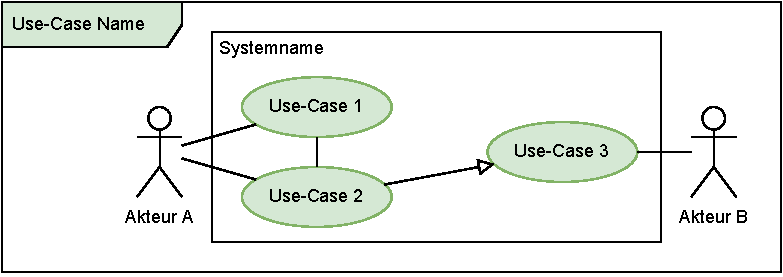
\includegraphics[width=\textwidth]{includes/figures/02_use_case_diagram.pdf}

    Anbei findet man eine tabellarische textuelle Beschreibung jedes relevanten Anwendungsfalls:

    \begin{tabularx}{\textwidth}{|>{\bfseries}l|X|}
        \hline
        \multicolumn{2}{|l|}{Use-Case-Nummer, Use-Case-Name}                                                                                                 \\\hline\hline
        Kurzbeschreibung  & ein kurzer erklärender strukturierter Satz zur Übersicht                                                                         \\\hline
        Akteure           & Personen bzw. Rollen oder externe Systeme, die aktiv mit dem System interagieren oder einen Nutzen von dem Anwendungsfall haben.
        Ein Anwendungsfall kann mit mehreren Akteuren verbunden sein.                                                                                        \\\hline
        Kategorie         & muss, soll oder kann der Anwendungsfall realisiert werden                                                                        \\\hline
        Auslösung         & ein Akteur oder eine Funktion, die den Ablauf startet                                                                            \\\hline
        Vorbedingung      & eine Bedingung, die erfüllt sein muss, damit der Ablauf gestartet wird                                                           \\\hline
        Eingabe / Ausgabe & für den Ablauf benötigte Informationen / Ergebnis des Ablaufs                                                                    \\\hline
        Nachbedingung     & Eine Bedingung, die erfüllt sein muss, um den Anwendungsfall zu beenden                                                          \\\hline
        Ablauf            & beschreibt den Standardablauf - keine Sonderfälle                                                                                \\\hline
    \end{tabularx}
\end{defi}

\begin{defi}{Akteur (Use-Case-Diagramm)}
    \begin{wrapfigure}{r}{0.15\textwidth}
        \begin{center}
            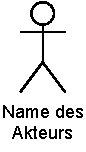
\includegraphics[width=0.1\textwidth]{includes/figures/02_akteur.pdf}
        \end{center}
    \end{wrapfigure}

    Personen oder Rollen werden meist durch Akteure beschreiben.

    In Use-Case Diagrammen stoßen diese Akteure Anwendungsfälle an.

    Alternativ stehen neben dem stilisiertem Symbol weitere Rollen-spezifische Symbole zur Verfügung:

    \begin{center}
        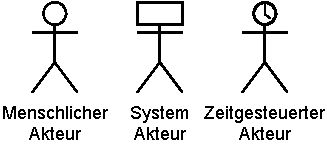
\includegraphics[width=0.4\textwidth]{includes/figures/02_akteur_types.pdf}
    \end{center}
\end{defi}

\begin{bonus}{Spezifischer Akteur (Use-Case-Diagramm)}
    \begin{wrapfigure}{r}{0.35\textwidth}
        \begin{center}
            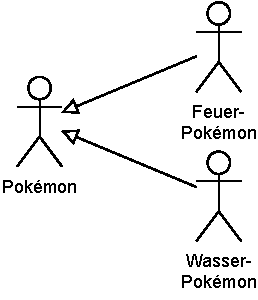
\includegraphics[width=0.3\textwidth]{includes/figures/02_akteur_specification.pdf}
        \end{center}
    \end{wrapfigure}

    Wenn Akteure durch bestimmte Eigenschaften erweitert werden müssen, jedoch in ihrer Grundform weiterhin benötigt werden, kann man diese spezifische Rollen durch allgemeinen Rollen generalisieren\footnote{Vergleichbar mit Vererbung in objektorientierter Programmierung}.

    Dementsprechend wird hier der Akteur \emph{Pokémon} durch \emph{Feuer-} sowie \emph{Wasser-Pokémon} spezialisiert.

    \vspace{1.5cm}
\end{bonus}

\begin{defi}{Use-Case (Use-Case-Diagramm)}
    \begin{wrapfigure}{r}{0.25\textwidth}
        \begin{center}
            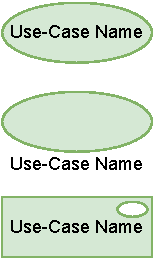
\includegraphics[width=0.2\textwidth]{includes/figures/02_use_case.pdf}
        \end{center}
    \end{wrapfigure}

    \emph{Use-Cases} bzw. Anwendungsfälle beschreiben eine Aktivität.
    Dabei besteht der Name aus einem Substantiv und einem Verb.

    z.B. würde \enquote{Pokémon fangen} diese Namenskonvention erfüllen.

    Diese werden meist mit einem Oval oder einer Ellipse dargestellt.
    Dabei steht der Name - je nach vorhandenem Platz - entweder in dem Symbol oder darunter.

    \vspace{2cm}
\end{defi}

\begin{defi}{Systeme und Grenzen (Use-Case-Diagramm)}
    Um das Gesamtsystem aus fachlicher Sicht einzuordnen, kann man Anwendungsfalls-Gruppen in einem \emph{System} zusammenfügen.
    Diese Systeme grenzen verschiedene fachliche Teile, Aufgaben und/ oder Verantwortungsbereiche voneinander ab.

    %Dabei dient die Einteilung nicht als technische Analyse!
\end{defi}

\begin{defi}{Kanten bzw. Assoziationen (Use-Case-Diagramm)}
    \emph{Kanten bzw. Assoziation} modellieren Interaktionen zwischen:
    \begin{itemize}
        \item Akteur und Akteur
        \item Akteur und Use-Case
        \item Use-Case und Use-Case
    \end{itemize}
    und beantworten die Frage, wer mit wem in welcher Beziehung steht.

    Dabei erfolgt die Darstellung über Kanten und Linien, welche ggf. über Zusätzliche Annotationen angereichert werden.
\end{defi}

\begin{bonus}{Zusammenfassung Assoziationstypen (Use-Case-Diagramm)}
    \begin{itemize}
        \item Binäre Assoziation (ungerichtet)

              Richtung nicht eindeutig, i.d.R. ausgehend von einem der beteiligten Akteuren

              \vspace{1em}
              \begin{center}
                  
\includegraphics[width=0.5\textwidth]{includes/figures/02_assoziation.pdf}
              \end{center}

        \item Import/ Include Beziehung

              \emph{A} \emph{umfasst} das Verhalten von \emph{B} vollständig.
              D.h. B ist eine Teilfunktion von A.
              A beinhaltet aber noch weitere Teile.
              Dies ist eine klassische Anwendung um Redundanzen zu vermeiden:
              Mehrere Use-Cases führen denselben Teil aus, dann wird er ausgelagert und gemeinsam genutzt.

              \vspace{1em}
              \begin{center}
                  
\includegraphics[width=0.5\textwidth]{includes/figures/02_include.pdf}
              \end{center}

        \item Erweiterungsbeziehung

              \emph{A} \emph{erweitert} \emph{B} unter einer speziellen Voraussetzung

              \vspace{1em}
              \begin{center}
                  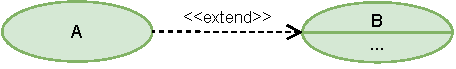
\includegraphics[width=0.5\textwidth]{includes/figures/02_extend.pdf}
              \end{center}

        \item Generalisierungsbeziehung

              \emph{A} ist ein \emph{B}.
              Interessant bei abstrakten Akteuren und / oder Teilsystemen.

              \vspace{1em}
              \begin{center}
                  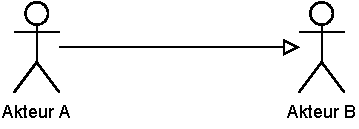
\includegraphics[width=0.4\textwidth]{includes/figures/02_generalisierung.pdf}
              \end{center}
    \end{itemize}

    Obacht: Bei der Angabe mehrerer Assoziationen ist die Reihenfolge nicht festgelegt.
\end{bonus}

\begin{example}{Use-Case-Diagramm}
    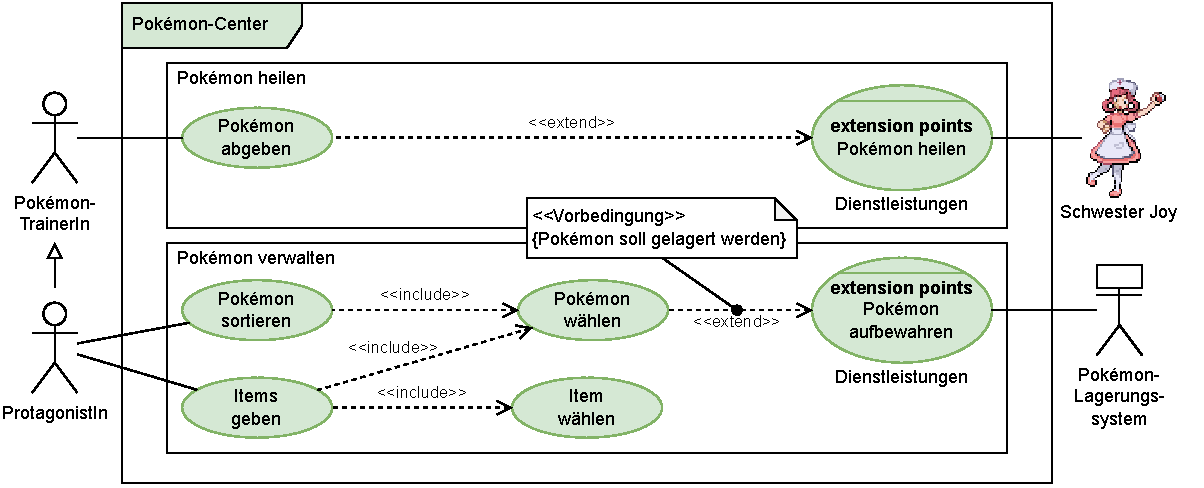
\includegraphics[width=\textwidth]{includes/figures/02_use_case_example.pdf}
\end{example}

\begin{example}{UC2: Use-Case-Diagramm (Textuelle Beschreibung)}
    \begin{tabularx}{\textwidth}{|>{\bfseries}l|X|}
        \hline
        \multicolumn{2}{|l|}{Pokémon sortieren}                                                                                \\\hline\hline
        Kurzbeschreibung  & Verwaltet das aktuelle Team und tauscht - falls nötig - Pokémon aus dem Pokémon-Lagerungsystem ein \\\hline
        Akteure           & ProtagonistIn                                                                                      \\\hline
        Kategorie         & kann                                                                                               \\\hline
        Auslösung         & Entscheidung das Team zu modifizieren                                                              \\\hline
        Vorbedingung      & mind. zwei Pokémon im Team bzw. in der Box vorhanden                                               \\\hline
        Eingabe / Ausgabe & E: Altes Team, Modifikation, A: Neues Team                                                         \\\hline
        Nachbedingung     & Pokémon wurden gewählt und getauscht                                                               \\\hline
        Ablauf            & \begin{enumerate}
                                \item ProtagonistIn betritt das Pokémon-Center
                                \item ProtagonistIn meldet sich am Pokémon-Lagerungsystem an
                                \item Solange ProtagonistIn nicht fertig
                                      \begin{enumerate}
                      \item Wähle auszutauschendes Pokémon
                      \item Wähle einzutauschendes Pokémon
                  \end{enumerate}
                            \end{enumerate}                                        \\\hline
    \end{tabularx}
\end{example}